\item A bobina tem uma massa de \SI{100}{\kilogram} e um raio de giração $k_{G}=\SI{.3}{\meter}$. Se os coeficientes de atrito cinético e estático em $A$ são $\mu_{s}=0.2$ e $\mu_{k}=0.15$, respectivamente, determine a aceleração angular da bobina se $P=\SI{600}{\newton}$

\import{../answers}{answer-15}

\begin{flushleft}
	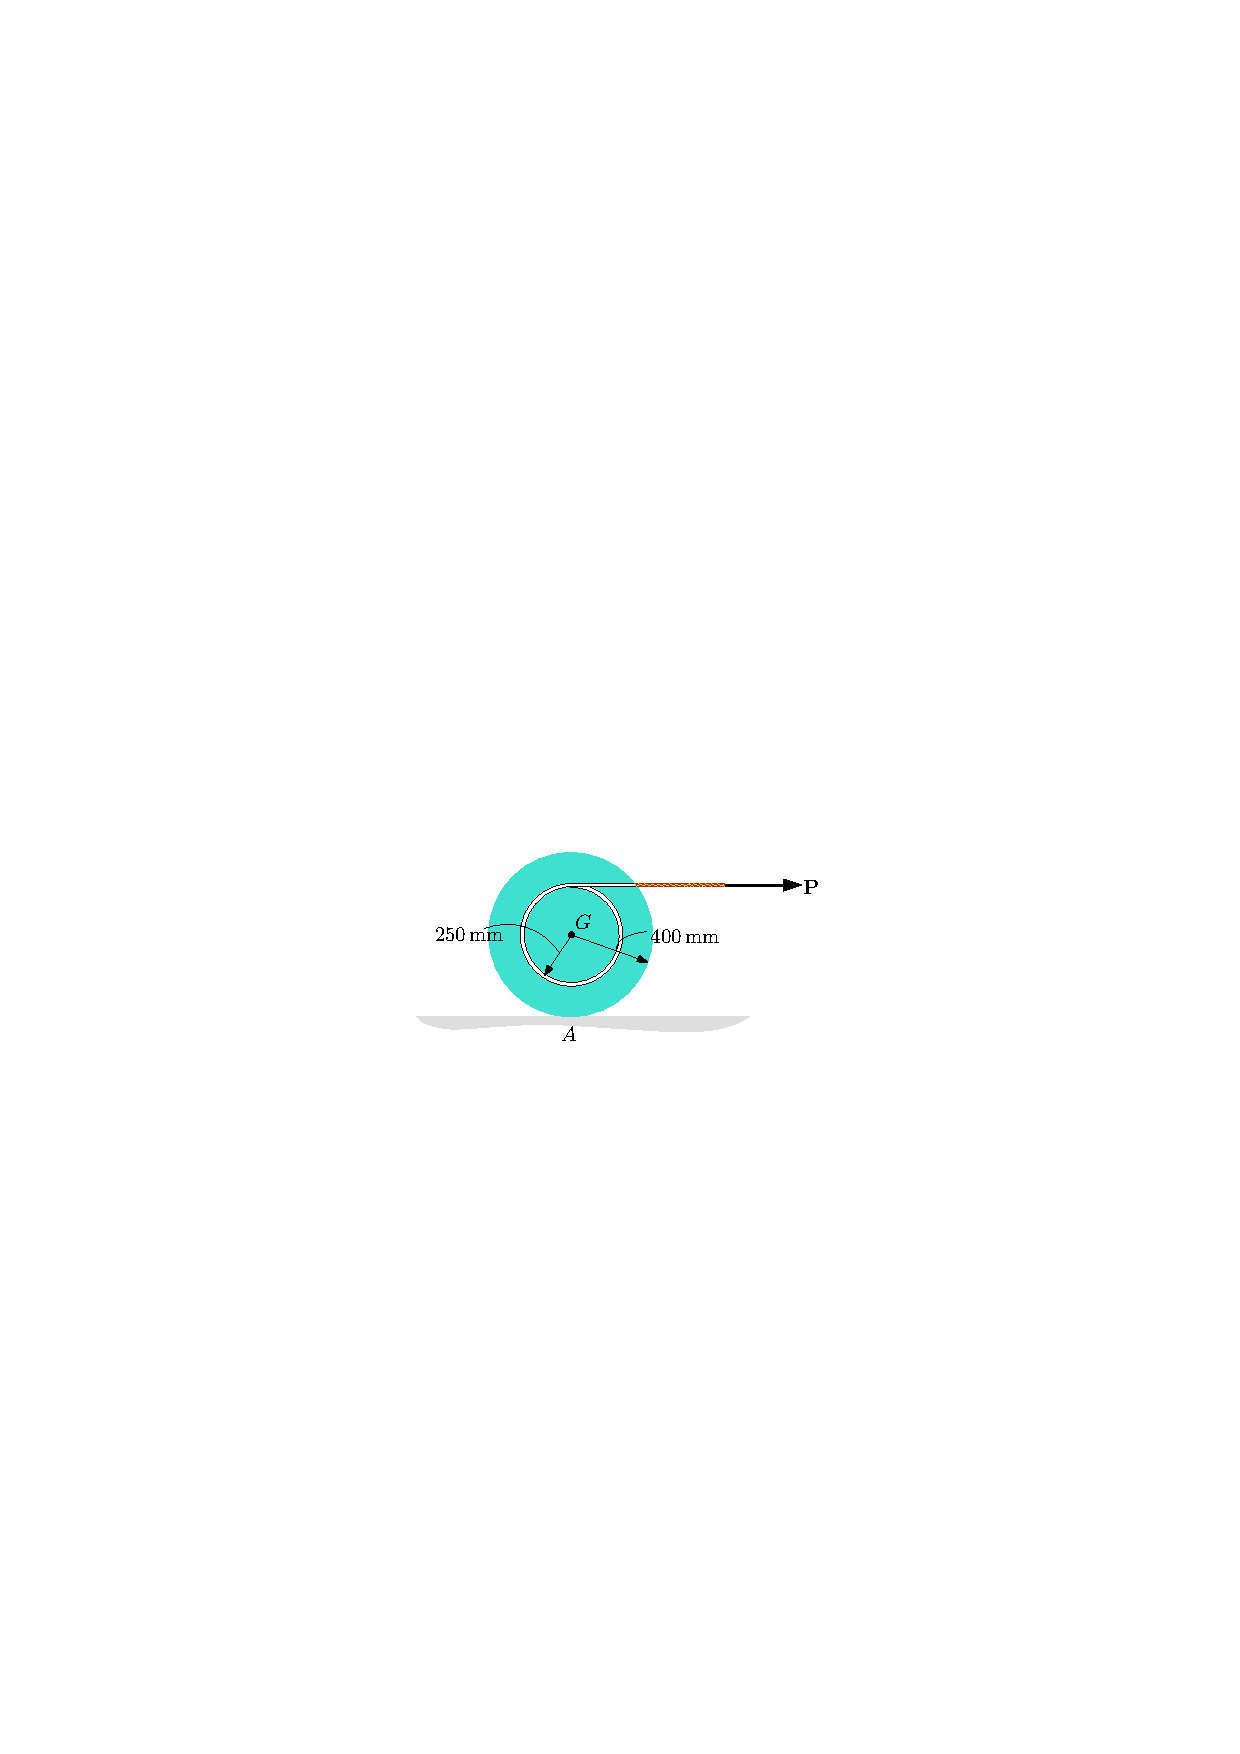
\includegraphics[scale=1.2]{../../images/draw_10_1}
\end{flushleft}